\section{A Novel Hilbert Antenna Enhanced With Metamaterials for Partial Discharge Detection}

\subsection*{Contexto y objetivo}
La detección de descargas parciales (PD, por sus siglas en inglés) es crucial para el mantenimiento y la seguridad de los equipos de alta tensión. Las antenas de ultra alta frecuencia (UHF) convencionales utilizadas para este fin adolecen de limitaciones significativas, como un tamaño físico excesivo y un ancho de banda estrecho. El presente estudio aborda estas limitaciones proponiendo un diseño novedoso de antena que busca expandir el ancho de banda sin aumentar las dimensiones físicas de la misma.

El objetivo principal de esta investigación es desarrollar una antena compacta con un ancho de banda amplio para la detección de PD en la banda UHF. Para lograrlo, se emplean dos estrategias:
\begin{enumerate}
    \item Integrar una curva fractal de Hilbert modificada en un diseño de antena espiral para ampliar el ancho de banda.
    \item Introducir una estructura de metamaterial simétrica de doble anillo abierto para mejorar aún más el rendimiento de la antena, incluyendo su ganancia, ancho de banda de detección y direccionalidad.
\end{enumerate}
La investigación busca validar el rendimiento de la antena propuesta tanto mediante simulaciones como experimentalmente.

\subsection*{Metodología o desarrollo}
El desarrollo de esta investigación se llevó a cabo en varias etapas, combinando el diseño de antenas fractales con metamateriales y su validación experimental.

\begin{enumerate}
    \item \textbf{Diseño de la antena espiral de Hilbert:}
    La antena espiral de Hilbert se diseñó integrando una curva fractal de Hilbert, conocida por sus propiedades de auto-similitud y llenado de espacio, en una disposición espiral rectangular. Esta integración permite excitar múltiples modos resonantes, ampliando el ancho de banda sin aumentar el tamaño físico.
    \begin{figure}[htpb]
    \centering
    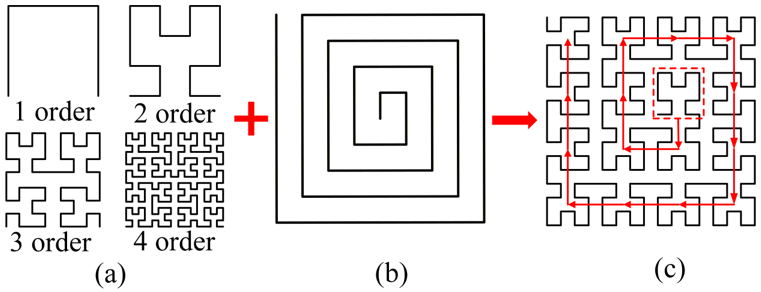
\includegraphics[width=0.8\textwidth]{images/80454576009ef7b4a427014bb7b6ca8c_p2_i1.png}
    \caption{Ideas de diseño para estructuras de antena espiral de Hilbert. (a) Curva de Hilbert. (b) Curva espiral rectangular. (c) Curva espiral de Hilbert.}
    \end{figure}
    Se realizó un estudio comparativo entre una antena espiral rectangular de 8 vueltas y una antena espiral de Hilbert de 2\textsuperscript{o} orden y 8 vueltas, ambas sobre un sustrato dieléctrico FR4 de 100 \texttimes\ 100 \texttimes\ 1.6 mm. Los resultados (ilustrados en \textbf{Figure 3}) mostraron que la antena espiral de Hilbert duplicaba el ancho de banda operativo (21.8\% vs. 9\%) para un VSWR $<$ 2.
    \begin{figure}[htpb]
    \centering
    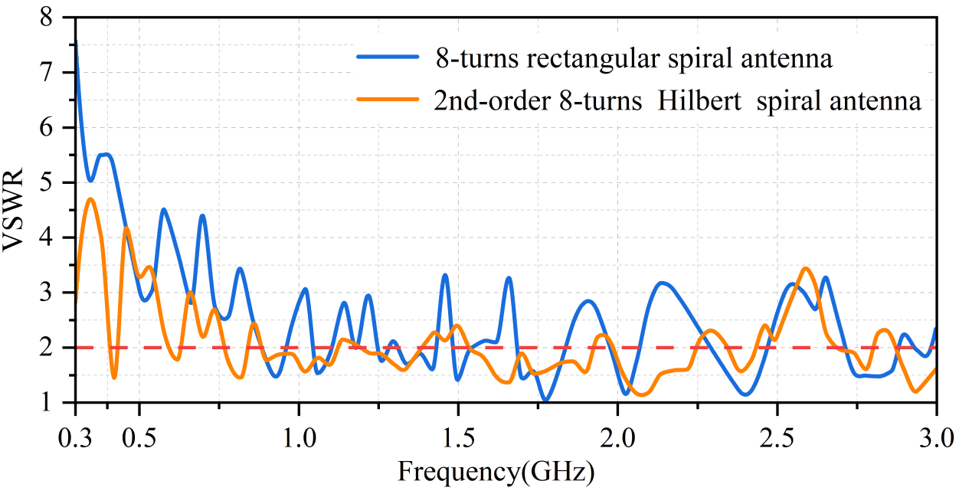
\includegraphics[width=0.8\textwidth]{images/80454576009ef7b4a427014bb7b6ca8c_p2_i2.png}
    \caption{Curvas de VSWR de la antena espiral de Hilbert de 2\textsuperscript{o} orden y ocho vueltas y la antena espiral rectangular de ocho vueltas.}
    \end{figure}
    A través de un análisis paramétrico de diferentes órdenes fractales y números de vueltas (detallado en \textbf{Table I} del documento original), se seleccionó la antena espiral de Hilbert de 2\textsuperscript{o} orden y cuatro vueltas como el diseño final, que ofrecía un ancho de banda operacional del 56.7\% en la banda UHF.

    \item \textbf{Diseño de la unidad de metamaterial:}
    Para mejorar el ancho de banda del 56.7\% de la antena espiral de Hilbert, se introdujo una estructura de metamaterial (MM) consistente en una unidad simétrica de doble anillo abierto con un diseño espiral continuamente curvado. Este diseño se basa en la teoría de resonancia LC (\textbf{ecuación 1} del documento), optimizando la inductancia y capacitancia equivalentes para reducir la frecuencia resonante fundamental sin aumentar el tamaño.
    \begin{figure}[htpb]
    \centering
    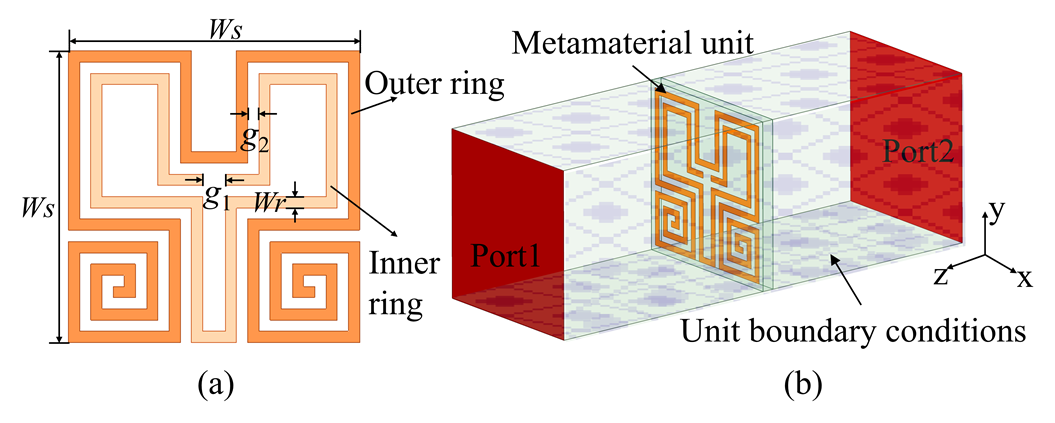
\includegraphics[width=0.8\textwidth]{images/80454576009ef7b4a427014bb7b6ca8c_p3_i1.png}
    \caption{(a) Estructura de la unidad de metamaterial y (b) esquema de simulación del puerto Floquet.}
    \end{figure}
    Las simulaciones electromagnéticas de onda completa se realizaron utilizando CST Studio Suite, aplicando el método de puerto Floquet. Se llevó a cabo una optimización paramétrica variando el ancho de línea (\textit{wr}), el ancho de la brecha interna (\textit{g1}) y el ancho de la brecha entre anillos (\textit{g2}) para analizar su influencia en la curva S21 (como se muestra en \textbf{Figure 5} del documento original, partes (a), (b) y (c)).
    \begin{figure}[htpb]
    \centering
    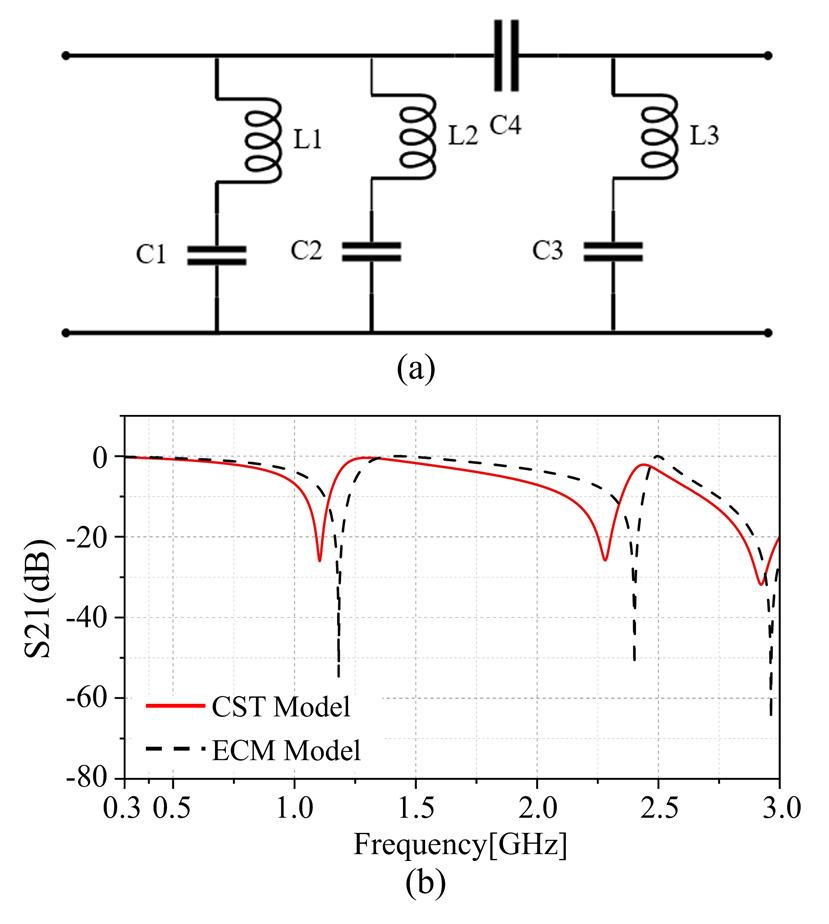
\includegraphics[width=0.8\textwidth]{images/80454576009ef7b4a427014bb7b6ca8c_p4_i1.png}
    \caption{Curva S21 obtenida al cambiar $w_r$.}
    \end{figure}
    \begin{figure}[htpb]
    \centering
    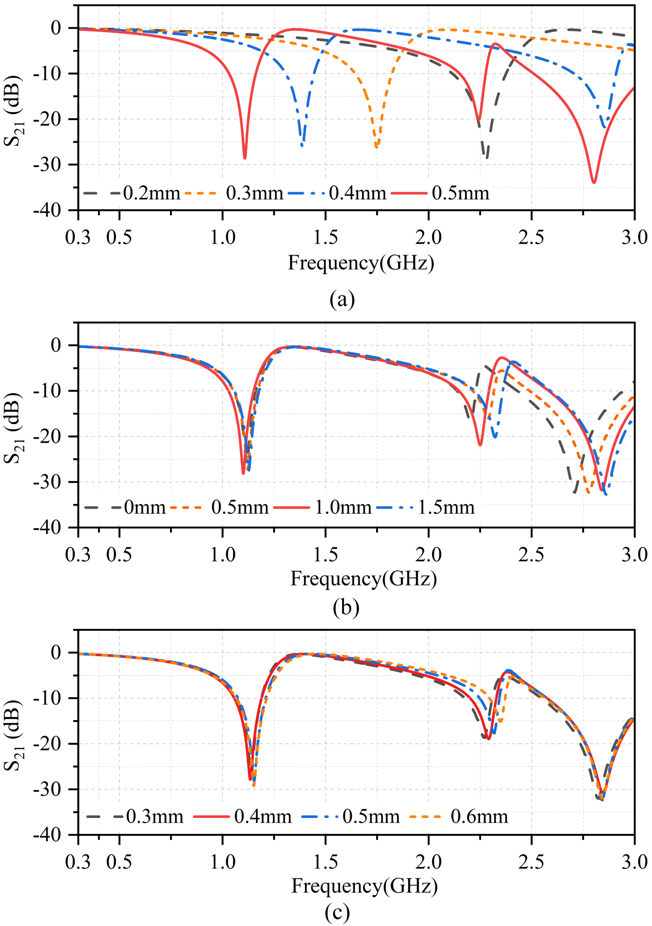
\includegraphics[width=0.8\textwidth]{images/80454576009ef7b4a427014bb7b6ca8c_p4_i2.png}
    \caption{Curva S21 obtenida al cambiar $g_1$.}
    \end{figure}
    \begin{figure}[htpb]
    \centering
    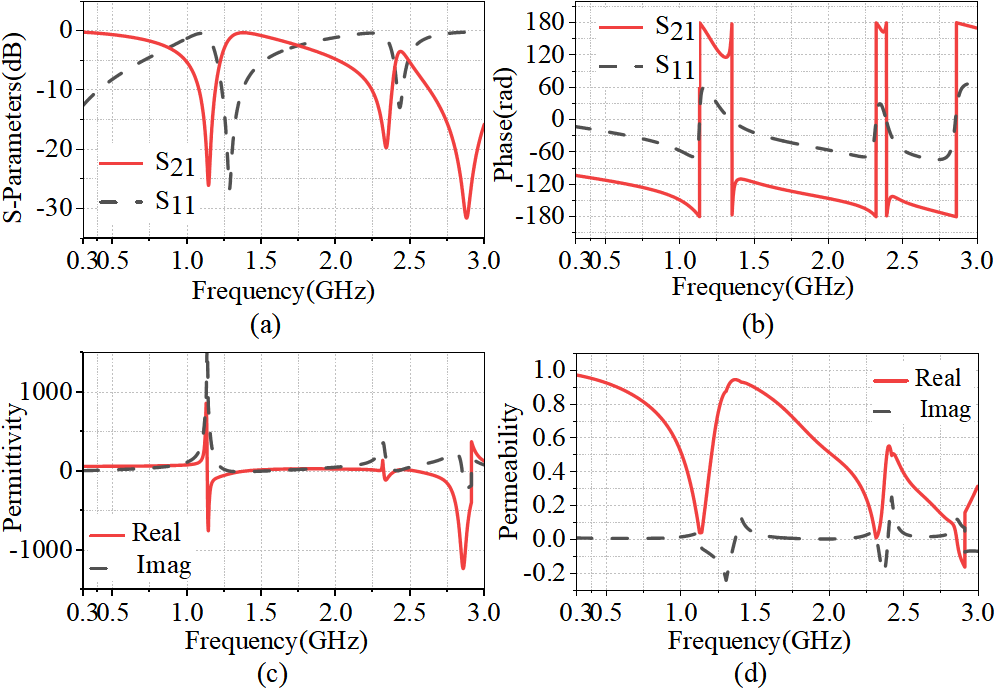
\includegraphics[width=0.8\textwidth]{images/80454576009ef7b4a427014bb7b6ca8c_p4_i3.png}
    \caption{Curva S21 obtenida al cambiar $g_2$.}
    \end{figure}
    Los parámetros finales optimizados fueron: $ws = 13$ mm, $wr = 0.5$ mm, $g1 = 1$ mm y $g2 = 0.4$ mm. Se desarrolló un modelo de circuito equivalente para caracterizar el mecanismo de transmisión de ondas electromagnéticas, validado por simulaciones de onda completa (detallado en \textbf{Figure 7} del documento original, que no se incluye en esta respuesta).

    \item \textbf{Integración de metamateriales en la antena:}
    El metamaterial se dispuso en un arreglo de 8 \texttimes\ 8 unidades a una altura $d_1$ por encima de la antena espiral de Hilbert, fabricado sobre un sustrato FR4. El principio es modificar la trayectoria de propagación de las ondas electromagnéticas, permitiendo que la antena capture más señales entrantes y mejore su sensibilidad (\textbf{Figure 8}).
    \begin{figure}[htpb]
    \centering
    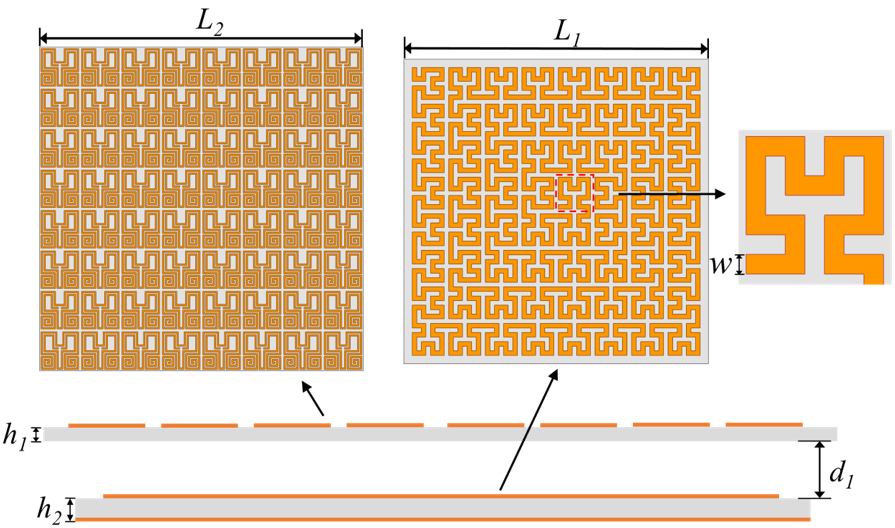
\includegraphics[width=0.8\textwidth]{images/80454576009ef7b4a427014bb7b6ca8c_p5_i1.png}
    \caption{Trayectoria de propagación de ondas electromagnéticas a través de la placa de metamaterial.}
    \end{figure}
    Se realizó una optimización de la distancia $d_1$ entre el arreglo de metamaterial y la antena, con simulaciones para $d_1$ = 10, 20, 30 y 40 mm (\textbf{Figure 10}). El valor óptimo de $d_1$ se determinó en 10 mm.
    \begin{figure}[htpb]
    \centering
    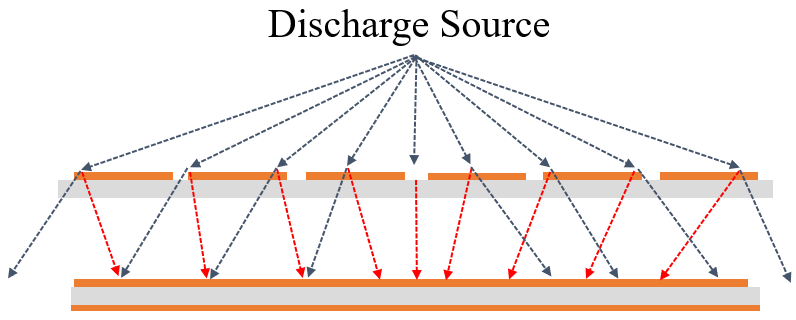
\includegraphics[width=0.8\textwidth]{images/80454576009ef7b4a427014bb7b6ca8c_p5_i2.png}
    \caption{Estructura general de la antena espiral de Hilbert con metamateriales.}
    \end{figure}
    \begin{figure}[htpb]
    \centering
    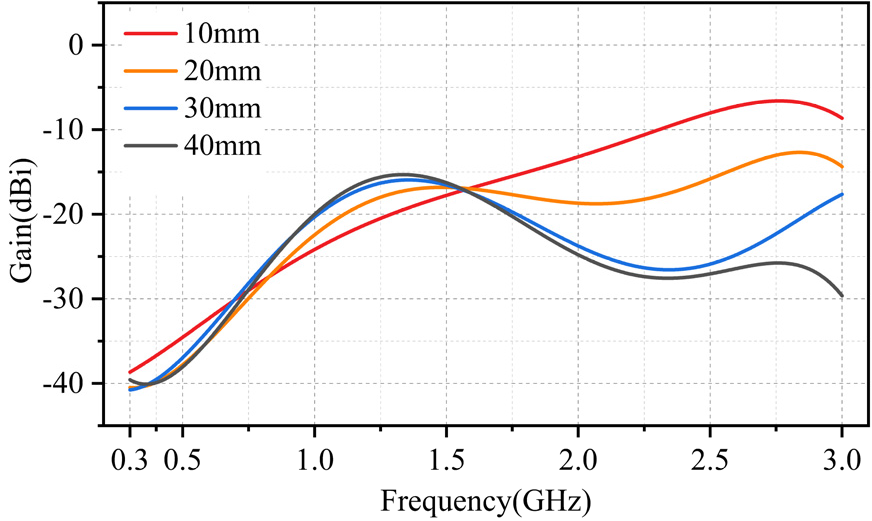
\includegraphics[width=0.8\textwidth]{images/80454576009ef7b4a427014bb7b6ca8c_p5_i3.png}
    \caption{Ganancia a diferentes distancias entre el arreglo de metamaterial y la antena.}
    \end{figure}

    \item \textbf{Pruebas de antenas y metamateriales:}
    Tras las simulaciones, la antena diseñada y el arreglo de metamaterial se fabricaron en una placa de circuito impreso (PCB). Se validó experimentalmente su rendimiento utilizando el método de medición en espacio libre para los parámetros S, VSWR y ganancia. El sistema experimental (\textbf{Figure 14}) utiliza una antena transmisora, la placa de metamaterial, la antena receptora y un analizador vectorial de redes (VNA).
    \begin{figure}[htpb]
    \centering
    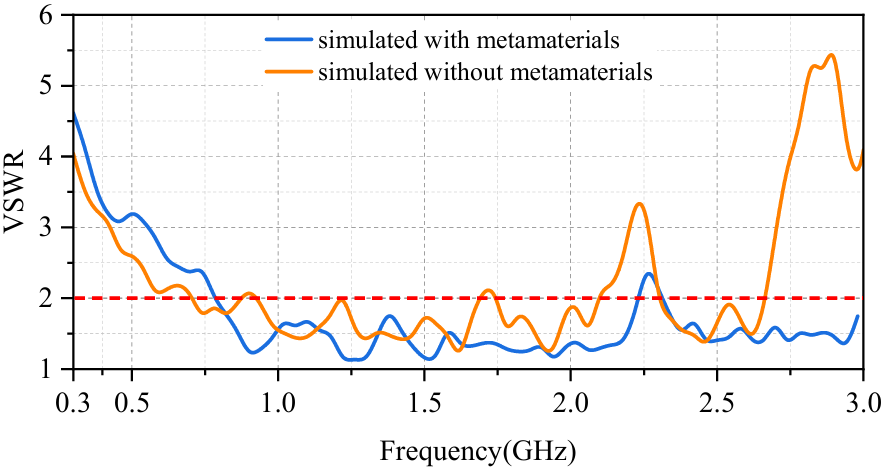
\includegraphics[width=0.8\textwidth]{images/80454576009ef7b4a427014bb7b6ca8c_p6_i4.png}
    \caption{(a) Medición de parámetros S de metamateriales por el método de espacio libre. (b) Diagrama de medición in situ por el método de espacio libre.}
    \end{figure}
    Finalmente, se construyó un sistema de detección de PD en laboratorio para evaluar la capacidad de la antena de detectar señales de PD. Este sistema (\textbf{Figure 18}) incluía un transformador, un resistor limitador, un aislante compuesto (contaminado artificialmente), un osciloscopio y dos antenas (con y sin metamateriales), junto con amplificadores de bajo ruido.
    \begin{figure}[htpb]
    \centering
    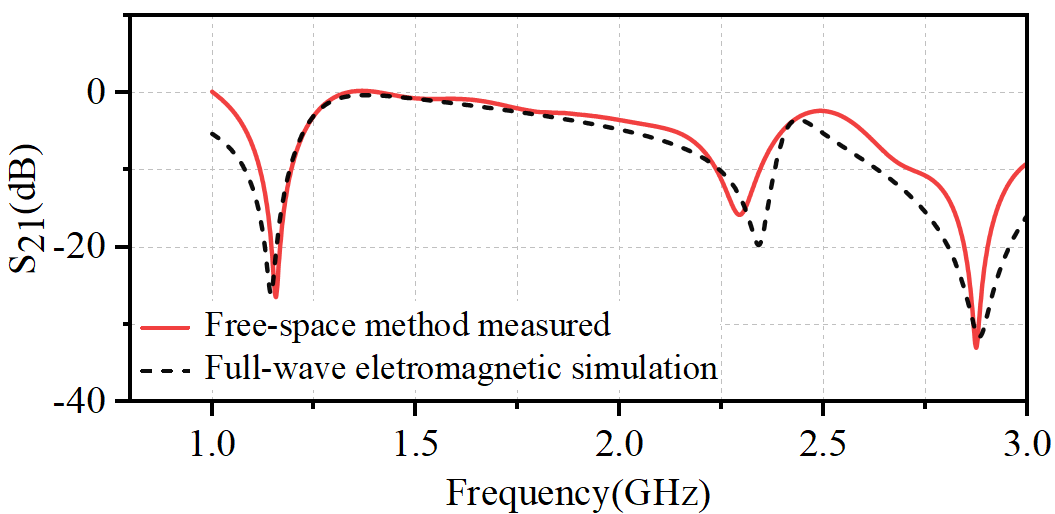
\includegraphics[width=0.8\textwidth]{images/80454576009ef7b4a427014bb7b6ca8c_p7_i8.png}
    \caption{(a) Diagrama del sistema de detección de PD.}
    \end{figure}
    \begin{figure}[htpb]
    \centering
    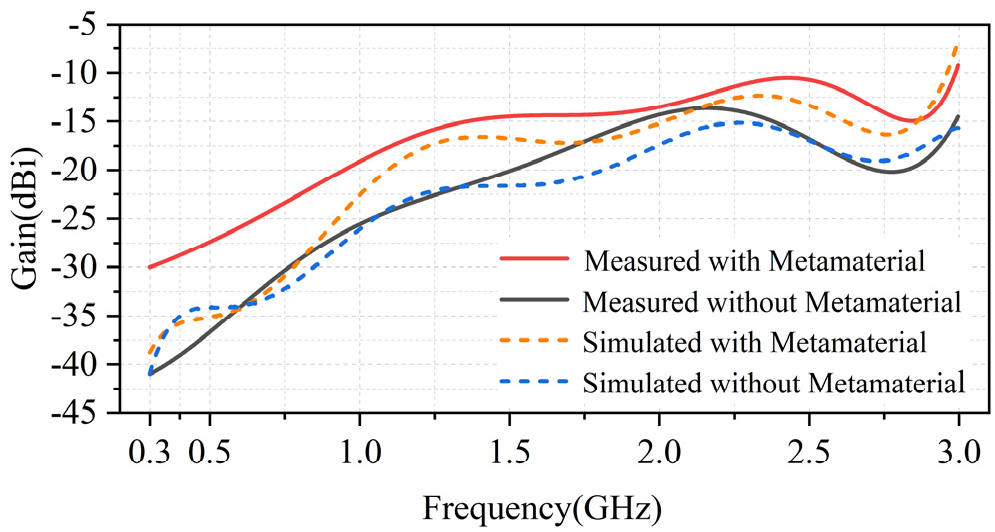
\includegraphics[width=0.8\textwidth]{images/80454576009ef7b4a427014bb7b6ca8c_p7_i9.png}
    \caption{(b) Disposición del sitio experimental.}
    \end{figure}
    \begin{figure}[htpb]
    \centering
    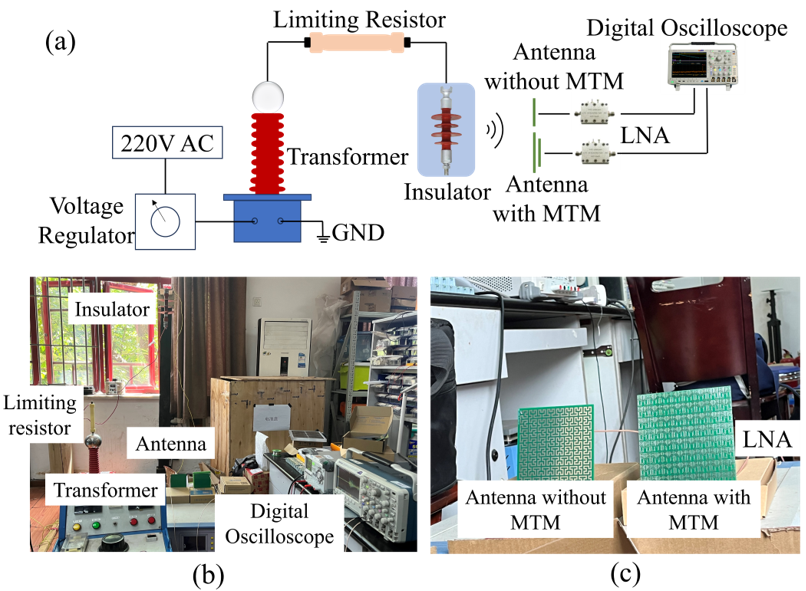
\includegraphics[width=0.8\textwidth]{images/80454576009ef7b4a427014bb7b6ca8c_p7_i10.png}
    \caption{(c) Disposición de la antena en el experimento de campo.}
    \end{figure}
    Se midieron las señales de PD a diferentes distancias (2-10 m) para ambas configuraciones de antena (con y sin metamateriales), y se calcularon las amplitudes de pulso promedio (APA) para cuantificar la sensibilidad de detección (según la \textbf{ecuación 8} del documento).
\end{enumerate}

\subsection*{Resultados o hallazgos}
Los resultados de este estudio demuestran mejoras significativas en el rendimiento de la antena:
\begin{enumerate}
    \item \textbf{Antena espiral de Hilbert (diseño base):} El diseño de 2\textsuperscript{o} orden y 4 vueltas de la antena espiral de Hilbert logró un ancho de banda operativo del 56.7\% en la banda UHF para un VSWR $<$ 2.

    \item \textbf{Rendimiento de la unidad de metamaterial:} La unidad de metamaterial exhibió tres ceros de transmisión a 1.1, 2.25 y 2.9 GHz. Mostró permisividad negativa en rangos de frecuencia de 1.13-1.35 GHz, 2.32-2.39 GHz y 2.56-2.91 GHz, y simultáneamente permisividad y permeabilidad negativas en el rango de 2.86-2.91 GHz. El modelo de circuito equivalente desarrollado se validó con éxito mediante simulaciones de onda completa (resultados de la \textbf{Figure 6} y \textbf{Figure 7} del documento original, no incluidas en esta respuesta).

    \item \textbf{Antena con metamateriales (simulación):}
    \begin{figure}[htpb]
    \centering
    \includegraphics[width=0.8\textwidth]{images/80454576009ef7b4a427014bb7b6ca8c_p11_i1.png}
    \caption{VSWR de diferentes antenas.}
    \end{figure}
    Comparando la antena sin y con metamateriales, la configuración integrada logró un VSWR $<$ 2 en dos bandas de frecuencia amplias: 0.78-2.02 GHz y 2.22-3 GHz. Esto representa un aumento del 24.4\% en el ancho de banda operacional. Se observó una mejora promedio de la ganancia de 4.61 dBi (\textbf{Figure 10}). La directividad y el rendimiento de radiación se vieron significativamente mejorados, con una concentración de la energía radiada (\textbf{Figure 12}).
    \begin{figure}[htpb]
    \centering
    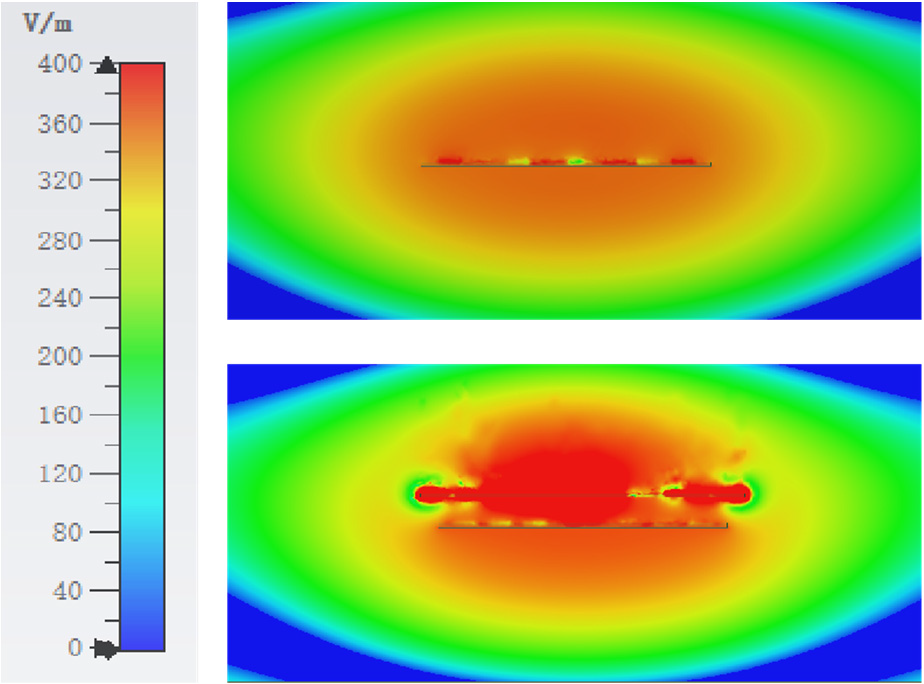
\includegraphics[width=0.8\textwidth]{images/80454576009ef7b4a427014bb7b6ca8c_p6_i2.png}
    \caption{Dirección de radiación con y sin metamateriales de mejora a 1.1, 2.25 y 2.9 GHz.}
    \end{figure}
    La distribución del campo eléctrico (\textbf{Figure 13}) mostró que el metamaterial concentra y refuerza eficazmente el campo eléctrico, optimizando la trayectoria de propagación de ondas electromagnéticas y mejorando la eficiencia de radiación.
    \begin{figure}[htpb]
    \centering
    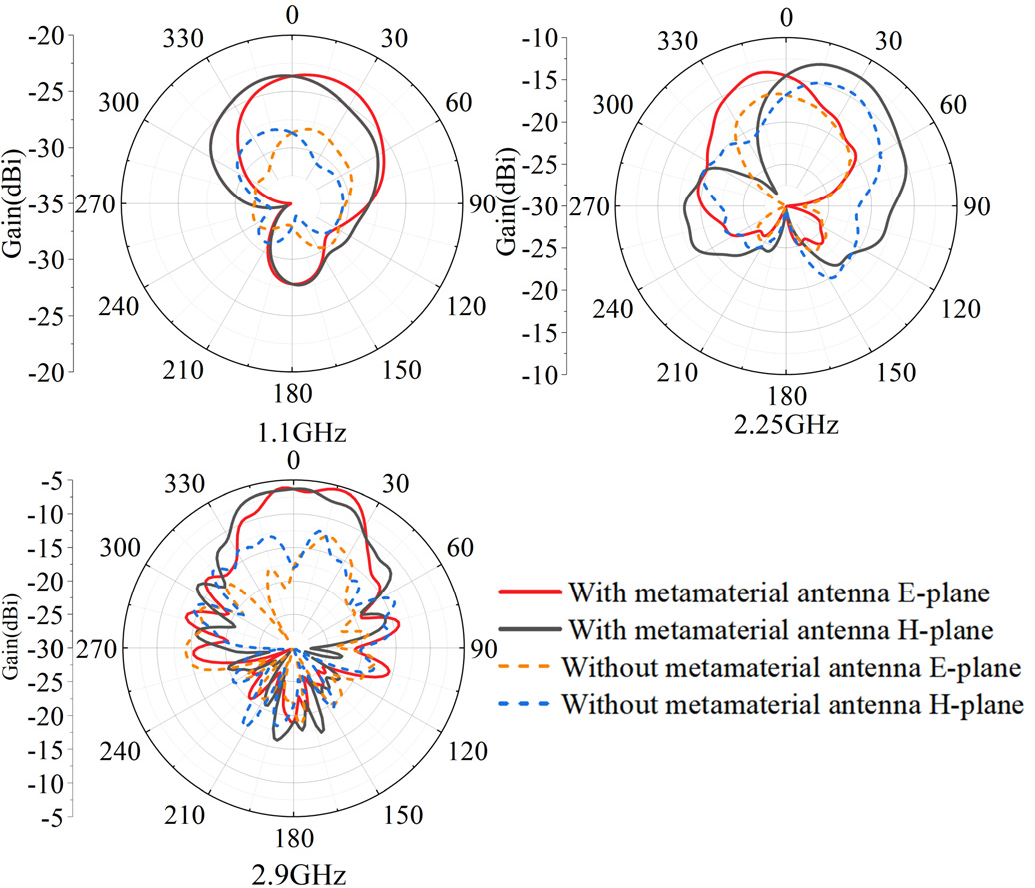
\includegraphics[width=0.8\textwidth]{images/80454576009ef7b4a427014bb7b6ca8c_p6_i3.png}
    \caption{Distribución del campo eléctrico con y sin metamaterial.}
    \end{figure}

    \item \textbf{Resultados de la validación experimental:}
    Las mediciones en espacio libre del parámetro S21 confirmaron la precisión de las simulaciones. Las curvas de VSWR y ganancia experimentales (mostradas en las \textbf{Figure 16} y \textbf{Figure 17} del documento original, no incluidas en esta respuesta) también se alinearon con los resultados simulados, validando el aumento del 24.4\% en el ancho de banda de detección y la mejora de la ganancia promedio de 4.61 dBi.
    En las pruebas de detección de PD (cuyas formas de onda y espectros de dominio temporal se presentan en las \textbf{Figure 19} y \textbf{Figure 20} del documento original, no incluidas aquí), la antena con metamateriales mostró una sensibilidad de detección 125\% mayor que la antena sin metamateriales a distancias de 2-8 m (según \textbf{Table III} del documento original). Además, el rango de detección de la antena con metamateriales se expandió hasta 10 m.
\end{enumerate}

\subsection*{Discusión o análisis crítico}
Este estudio aborda con éxito las limitaciones de tamaño y ancho de banda de las antenas UHF convencionales para la detección de PD. La integración de la curva fractal de Hilbert en el diseño espiral es una estrategia eficaz para lograr una mayor densidad de circuito y, por ende, un ancho de banda más amplio en un formato compacto. La naturaleza auto-similar y de llenado de espacio de los fractales de Hilbert permite resonancias multifrecuencia, lo que es esencial para cubrir el espectro amplio de las señales de PD.

La adición del metamaterial es la contribución clave para potenciar aún más el rendimiento de la antena. La estructura de doble anillo abierto con diseño espiral, operando bajo la teoría de resonancia LC, manipula eficazmente las ondas electromagnéticas. Al concentrar y reforzar el campo eléctrico, el metamaterial no solo amplía significativamente el ancho de banda y la ganancia, sino que también mejora la directividad de la antena. Esto se traduce en una mayor capacidad para capturar señales de PD, incluso débiles, y discernir su dirección.

La comparación con antenas reportadas en la literatura (\textbf{Table IV} del documento original) destaca que la antena propuesta es significativamente más compacta (100 \texttimes\ 100 \texttimes\ 1.6 mm) y logra un ancho de banda proporcional del 81.1\% en la banda UHF, superando la mayoría de los diseños existentes en términos de eficiencia de espacio y cobertura de frecuencia. Aunque la ganancia intrínseca de la antena es moderada debido a su tamaño compacto, la inclusión de amplificadores de bajo ruido en el sistema de detección compensa esta limitación, permitiendo un alcance de detección de 10 m.

Una limitación reconocida es que las pruebas experimentales se realizaron únicamente con aisladores. Sin embargo, el bajo coste de fabricación (sustrato FR4 y capa de microtira de cobre) y el diseño compacto la hacen atractiva para futuras aplicaciones de monitoreo en línea en equipos de alta tensión como GIS (sistemas de aislamiento de gas), transformadores y otros dispositivos complejos. La versatilidad de la matriz de metamateriales también sugiere su posible aplicación para mejorar otras antenas.

\subsection*{Conclusiones o implicaciones}
Este estudio presenta una solución innovadora y eficaz para la detección de descargas parciales (PD) en equipos de alta tensión. Se demuestra que la combinación de una antena espiral basada en la curva fractal de Hilbert y un arreglo de metamateriales es una estrategia robusta para superar las limitaciones de las antenas UHF convencionales.

El diseño de la antena espiral de Hilbert de 2\textsuperscript{o} orden y 4 vueltas es intrínsecamente compacto (100 \texttimes\ 100 \texttimes\ 1.6 mm) y proporciona un ancho de banda operativo del 56.7\%. La integración de un arreglo de metamateriales de doble anillo abierto y simétrico, colocado 10 mm por encima de la antena, amplía este ancho de banda en un 24.4\%, abarcando las bandas de 0.78-2.02 GHz y 2.22-3 GHz. Esta configuración también mejora la ganancia promedio en 4.61 dBi y aumenta la directividad, concentrando la energía del campo eléctrico y optimizando la trayectoria de propagación de las ondas.

Los resultados experimentales validan las simulaciones, mostrando una sensibilidad de detección 125\% mayor y un rango de detección extendido a 10 m para la antena con metamateriales, en comparación con el diseño sin metamateriales. Estas características la hacen altamente adecuada para el monitoreo en línea de PD, especialmente en espacios confinados como los encontrados en los GIS. La metodología y los hallazgos tienen implicaciones significativas para el desarrollo de futuras tecnologías de detección de PD más eficientes y compactas.

\subsection*{Síntesis final}
Este estudio presenta una antena espiral de Hilbert innovadora y compacta para la detección de descargas parciales (PD). La integración de un arreglo de metamateriales de doble anillo abierto mejora significativamente el ancho de banda en un 24.4\%, la ganancia promedio en 4.61 dBi y la directividad. Las simulaciones y experimentos confirman una sensibilidad de detección 125\% mayor y un alcance de 10 m, haciendo de esta antena una solución prometedora para el monitoreo en línea de equipos de alta tensión.